%%
%% This is file `sample-vem.tex',
%% which is a modified version of `sample-sigconf.tex'.
%%
\documentclass[sigconf]{acmart} % The `anonymous' option is for double-blind review process.

\usepackage{multirow}
\usepackage[table,xcdraw]{xcolor}

\usepackage{mdframed}

\usepackage{listings}

\lstset{
  basicstyle=\ttfamily\small,
  keywordstyle=\color{blue},
  commentstyle=\color{gray},
  stringstyle=\color{green!50!black},
  showstringspaces=false,
  numbers=none,
  numberstyle=\tiny,
  breaklines=true,
  frame=single
}

\mdfsetup{skipabove=\topskip,skipbelow=\topskip}
\mdfdefinestyle{poistyle}{%
    frametitlerule=true,
}
\mdtheorem[style=poistyle]{poi}{Improvement}

%%
%% \BibTeX command to typeset BibTeX logo in the docs
\AtBeginDocument{%
  \providecommand\BibTeX{{%
    \normalfont B\kern-0.5em{\scshape i\kern-0.25em b}\kern-0.8em\TeX}}}


%% These commands are for a PROCEEDINGS abstract or paper.
% \acmConference[SBES'24]{Brazilian Symposium on Software Engineering}{September 30 -- October 04,  2024}{Curitiba, PR}

%%
%% end of the preamble, start of the body of the document source.


\settopmatter{printacmref=false} % This command was added for submissions to VEM
\setcopyright{none} % This command was added for submissions to VEM
\renewcommand\footnotetextcopyrightpermission[1]{} % This command was added for submissions to VEM

\begin{document}

%%
%% The "title" command has an optional parameter,
%% allowing the author to define a "short title" to be used in page headers.
\title{Kworkflow: a Linux kernel Developer Automation Workflow System}
%enviar email para os chairs para atualizarmos o título
\pagestyle{empty}

%%
%% The "author" command and its associated commands are used to define
%% the authors and their affiliations.
%% Of note is the shared affiliation of the first two authors, and the
%% "authornote" and "authornotemark" commands
%% used to denote shared contribution to the research.
\author{David Tadokoro}
\email{davidbtadokoro@usp.br}
\orcid{}
\affiliation{%
    \institution{University of São Paulo}
  % \institution{Universidade de São Paulo}
  % \state{São Paulo}
  \country{Brazil}
}

\author{Rodrigo Siqueira}
\email{siqueirajordao@riseup.net}
\orcid{}
\affiliation{%
    \institution{University of São Paulo}
  % \institution{Universidade de São Paulo}
  % \state{São Paulo}
  \country{Brazil}
}

\author{Paulo Meirelles}
\email{paulormm@ime.usp.br}
\orcid{0000-0002-8923-2814}
\affiliation{%
    \institution{University of São Paulo}
  % \institution{Universidade de São Paulo}
  % \state{São Paulo}
  \country{Brazil}
}




%%
%% By default, the full list of authors will be used in the page
%% headers. Often, this list is too long, and will overlap
%% other information printed in the page headers. This command allows
%% the author to define a more concise list
%% of authors' names for this purpose.
\renewcommand{\shortauthors}{Pilone et al.}

\begin{abstract}
  The Linux kernel is a central project to the Free/Libre and Open Source
  Software (FLOSS) ecosystem. Developers who interact with the kernel source
  code routinely face a variety of repetitive and error-prone tasks, including
  setting up testing environments, managing kernel configuration files,
  compiling with various toolchains, deploying to varied targets, and correctly
  submitting patches. These tasks, though essential, often require handcrafted
  scripts that become fragile, difficult to maintain, and disconnected from the
  core development goals. Kworkflow (kw) is a Developer Automation Workflow
  System (DAWS) that aims to provide high-quality tools that mitigate known
  bottlenecks experienced by kernel developers in their daily workflows. It
  provides a unified Command-Line Interface (CLI) that automates and streamlines
  many tasks, allowing practitioners to focus more on developing code and less
  on setup overhead and details. The hub-like design of the project reflects its
  philosophy of incorporating existing tools to avoid duplication of efforts and
  wasted resources from the community, a by-product of the many \textit{ad-hoc}
  scripts developers commonly produce. The kw tool also offers a data collection
  infrastructure, which makes it an excellent platform for further scientific
  research in the Linux kernel development model. In this sense, kw serves as a
  robust tool for real kernel developers and an opportunity for academic
  research work.
\textbf{\href{https://archive.softwareheritage.org/swh:1:cnt:3695bf04c525dc03d850baa96485d7bcdca7f9b3;origin=https://github.com/davidbtadokoro/sbes-tool-2025-kw-demo;visit=swh:1:snp:21a2e8110b4a8c659c6ba451723f836d9fbba8db;anchor=swh:1:rev:1cef3fedffb5a4848bfe8f337cf1acd1380a7793;path=/sbes-tool-2025-kw-demo.mp4}{Link to the Kworkflow demo video}}~\cite{kw-demo-video}.
\end{abstract}


%%
%% Keywords. The author(s) should pick words that accurately describe
%% the work being presented. Separate the keywords with commas.
\keywords{Linux, Free Software, Linux kernel development model, Free Software development model, software engineering, kernel workflows.}

% \received{2 June 2024}
% \received[revised]{12 March 2009}
% \received[accepted]{5 June 2009}

%%
%% This command processes the author and affiliation and title
%% information and builds the first part of the formatted document.
\maketitle

\section{Introduction}

As a software solution, the Linux kernel is highly customizable and is on the
cutting edge of diverse fields, including Internet infrastructure, embedded
systems, cloud computing, and machine learning, making it critical for solving
real-world problems of society at large. 

When looking at the Linux kernel community from its data points, it is safe to
conclude that this project is one of the most thriving Free/Libre Open-Source
Software (FLOSS) projects by many metrics, such as the volume of volunteer
developers worldwide or the number of companies that invest in the project. The
Linux community has brought many people worldwide from different cultures,
beliefs, time zones, and others together to improve the project.\looseness=-1

Even though the project has been successful for over thirty years, it is still
evolving from the software engineering perspective. For example, due to its
size, the kernel requires developers to follow multiple processes and practices
that compose many workflows, some of which have associated bottlenecks that slow
down development; in this sense, newcomers need some time to get used to the
basic workflows, but even more experienced developers forget some aspects of the
development model and make mistakes. This is natural and, in some way, expected
when considering the vastness of the Linux kernel.

To mitigate workflow bottlenecks of large FLOSS projects, communities create
tools to streamline and automate their tasks. In the case of Linux, tools like
\texttt{get\_maintainers.pl}, \texttt{checkpatch.pl}, and
\texttt{git-send-email} help in the tasks of finding the correct recipients to
send contributions, checking for code style violations, and distributing patches
(code changes) via email, respectively. It is worth noting that configuring
these tools is often a complex and time-consuming chore by itself.

The main point is that multiple tools maintained inside and outside the Linux
project support the many kernel workflows. Beyond more consolidated and widely
adopted tools, for instance, the ones maintained inside the project's codebase
in the \texttt{scripts/} directory, it is commonplace for practitioners to
develop \textit{ad-hoc} scripts highly coupled with their development contexts
as solutions to gaps in the workflows not yet covered by existing tools or to
configuration overheads. As the primary goal of Linux developers is not to
develop and maintain supporting tools, these local solutions (although helpful)
duplicate community efforts and pulverize their resources, which could be spent
on fostering robust, high-quality collaborative tools.\looseness=-1

In other words, although many solutions cover many parts of the kernel
workflows, they are not unified, sometimes involve considerable effort to
configure, and are often unknown outside specific development contexts. All
Linux developers - contributors or maintainers, newcomers or veterans - would
benefit from a project that robustly integrates these solutions and implements
novel ones, presenting a hub-like interface that comprehensively abstracts the
kernel workflows.\looseness=-1

With all those ideas in mind, and considering that the described tools are
invaluable to maintaining a large-scale project like the Linux kernel, to the
point that they are crucial for its long-term
sustainability~\cite{corbet-gregkh2017-linuxreport}, this paper presents a set
of tools in a unified interface called \textit{Kworkflow} (kw), that streamlines
and automates the many kernel workflows while enforcing the project rules.

%%% TODO: SHOULD WE INCLUDE THE MICRO-DEVOPS DISCUSSION? %%%
% With all those ideas in mind, this paper argues for the rise of a new set of
% micro-DevOps tools that emerge from complex projects focused on ensuring that
% the project is maintainable and scalable for all levels of developers. This work
% was conducted over the years by creating an actual tool that intends to unify
% the kernel workflow in a single tool, enforcing the project rules in a
% low-effort way for experienced developers and newcomers.

\section{Background}

The FLOSS dynamics are incredibly diverse, and each project, including the Linux
kernel, has unique complexities. This section is dedicated to unraveling the
intricate concepts of kernel development and providing a solid foundation for
the ideas presented in this paper.

It is essential to highlight that Linux is an operating system kernel that runs
on multiple hardware configurations and has an extensive domain scope. To give
the development model scalability, the project is broken down into sub-projects
called subsystems, each with its particular focus, community, rules, and
(generally) dedicated git repository (called \textit{kernel tree}). Even inside
the subsystems, more specific development contexts can recursively partition the
subsystem into smaller sub-projects, although the recursion usually does not go
deep~\cite{corbet2017-patchflow}.

This dynamic forms a hierarchy in the shape of an umbrella, where maintainers of
a given kernel tree receive patches from contributors and, upon approval, send
them to the upper levels of the hierarchy: either the \textit{mainline} that is
the tree at the top of the hierarchy representing the top level Linux project or
a mid-level tree. This structure is reminiscent of a FLOSS equivalent to a city
divided into neighborhoods~\cite{wen2021-masterthesis}. The hierarchy is held
together as a \textit{web of trust}~\cite{corbet2014-4.4}, where upper levels
trust that lower levels will send correct contributions in the project's
standard, avoiding duplication of code-reviewing efforts, and allowing
highly-specialized personnel in all parts of the project. 

For instance, the \textit{Direct Rendering Management} (DRM) subsystem
encapsulates all device drivers associated with GPUs. In DRM, multiple vendors
maintain their drivers in their trees. In this scenario, a given vendor
specialized in its respective drivers will have a dedicated kernel tree that
accepts contributions and feeds them to DRM. In turn, DRM will integrate and
stabilize all contributions from all its sources and feed them to the mainline. 

In reality, the Linux development model is much more complex, involving strict
release cycles, \textit{Continuous Integration} (CI) workflows, stable releases,
and more. Nevertheless, the previous description gives us the necessary
information to understand the overarching project's dynamics.

\subsection{Fundamental tasks of Linux developers}
\label{sec:background:linux-tasks}

Linux kernel workflows are composed of fundamental tasks, with some being more
technical than others. Next, we highlight some of them.

The most common task that a kernel developer has to deal with daily is compiling
the kernel from the source code, which is called \textit{building} the kernel.
Unlike other projects that need compilation, this is not trivial in the Linux
context. Linux is widespread and runs on virtually any type of commercial
processor; x86, PowerPC, ARM, MIPS, and RISC-V are a few of the architectures
supported. Other details deepen the complexity of the build task, for instance:
processors can support 16, 32, and 64-bit architectures; there are different
compilation toolchains like \texttt{GCC} and \texttt{Clang}; some cases require
cross-compilation techniques. To top it all, some developers need to compile the
same source code to different targets, resulting in different environments that
are hard to manage. Noteworthy is the fact that compiling a kernel is a
CPU-bound task that can take minutes to hours, even when allocating all the CPU
cores of a machine with considerable computational power.

Another fundamental task is installing the necessary artifacts from a kernel
build into a target machine and making the custom kernel bootable for
validation, also called \textit{deploying} a kernel. The target device can be
many things, such as a virtual machine running in the developer's host, another
machine connected via network or serial cable, or even the host machine where
the developer built the kernel. To deploy a kernel, the developer must consider
these details and also deal with bootloader configuration, distro-specific
behavior, and other minor details, like the precise placement of artifacts.

To manage all the possible build configurations, Linux uses a file named
\texttt{.config} that, essentially, describes which features and modules to
compile and how. Producing the correct \texttt{.config} for a given purpose
relies on many details, just like deploying a kernel, and developers usually
have a set of \texttt{.config} files that they need to manage manually. This
file is precious for developers since it can (among other things) be optimized
for specific target machines, reducing compilation time.

Finally, an important task is to send a patch to the maintai-ners/reviewers and
mailing lists, which involves more than resolving the recipients, such as
ensuring the message follows a rigid formatting, having a standardized preamble
in the subject, and other obligatory practices.

Notably, Linux developers have to be proficient in interacting with their
computer systems through the \textit{Command-Line Interface} (CLI), commonly
using an OS shell compatible with \textit{Bourne-Again Shell} (Bash). Not only
are some shell scripts part of the Linux code base, but a significant portion of
the work of a Linux developer, besides writing code, involves issuing commands
in a terminal. Some of them, like \textit{GNU Make} commands, demand many
options and/or arguments in a specific order, which becomes error-prone and
inefficient with repetition, even for veteran developers.

\subsection{Tools that support the Linux development}

Several tools have been created in the Linux context to mitigate workflow
bottlenecks, sometimes gaining so much traction that they result in a broader
public adoption. A prime example of a now project-agnostic tool initially
devised in the Linux context by its creator, Linus Torvalds, is
\texttt{git}~\cite{git}~\footnote{All software cited in this paper includes a
permalink to its archive on \textit{Software Heritage} (SWH), a platform for
collecting, preserving, and sharing source code with precise references down to
individual file fragments.}.

We can split the tools supporting kernel developers into two categories:
officially supported and community-maintained. The former reside inside kernel
trees (usually in the \texttt{scripts/} directory) and have numerous people
caring for them. The latter set comprises any other tool not officially
supported, ranging from personal-use shell scripts that are never publicly
published to projects diligently maintained by developers (voluntarily or
sponsored) that have a considerable adoption by the community.

Regarding officially supported tools, we can highlight
\texttt{get\_main\-tainers.pl}~\cite{get-maintainer} and
\texttt{checkpatch.pl}~\cite{checkpatch}, which enforce the written
documentation in the actual code. Take \texttt{get\_maintainers.pl} first; this
tool matches the current changes in the patch against the target kernel tree
and, based on that, lets the developer know which mailing lists and developers
should become recipients. A tool like that improves the contributor's chance of
getting their code accepted by the maintainer.

On the other hand, \texttt{checkpatch.pl} helps developers evaluate whether
their changes violate code style rules described in the documentation and avoid
wasting review cycles on basic things. In other words, \texttt{checkpatch.pl}
helps developers comply with the code style rules and optimizes the review
cycle.

As mentioned before, \texttt{git} can also be considered a Linux tool, despite
its pervasiveness in any project, as it is paramount for most of the Linux
development model. In any case, it is worth emphasizing the
\texttt{git-send-email} command that integrates kernel trees to the email-based
communication of the project.

Going towards community-maintained projects, the \texttt{b4}~\cite{b4_swh} tool
helps maintainers work with patches available in the
\url{https://lore.kernel.org} public-inbox, an archive of most Linux mailing
lists that represents an on-demand approach to consuming the flow of messages
without needing to subscribe to lists actively.

To name a few other examples that are not necessarily exclusive to the Linux
context: \texttt{qemu}~\cite{qemu-project}, \texttt{vitrme-ng}~\cite{virtme-ng},
the \textit{DRM Maintainer Tools}~\cite{drm-maintainer-tools}, and the
\textit{LLVM Project Tools}~\cite{llvm-project}.

Regardless, most Linux tools are \textit{ad-hoc} scripts created by developers
to support their specific variations of the kernel workflows. Usually,
developers maintain this type of script in some git forge or, more often than
not, only locally; many companies also develop some of those tools and maintain
them only for internal use. This fragmentation leads to many duplicated efforts
and wasted opportunities to scale the productivity of the Linux community.

\subsection{Patchset development and reviewing workflows}

% TODO: Corrigir referências a imagens
Two core and overall kernel workflows are the \textit{patchset development
workflow} (\textbf{Figure 1}) and the \textit{patchset reviewing workflow}
(\textbf{Figure 2}), which are more related to the work of contributors and
maintainers, respectively. A \textit{patchset} is a set of patches related by an
overarching context that are submitted together and represent a contribution.

\begin{figure}[ht]
    \centering
    \fbox{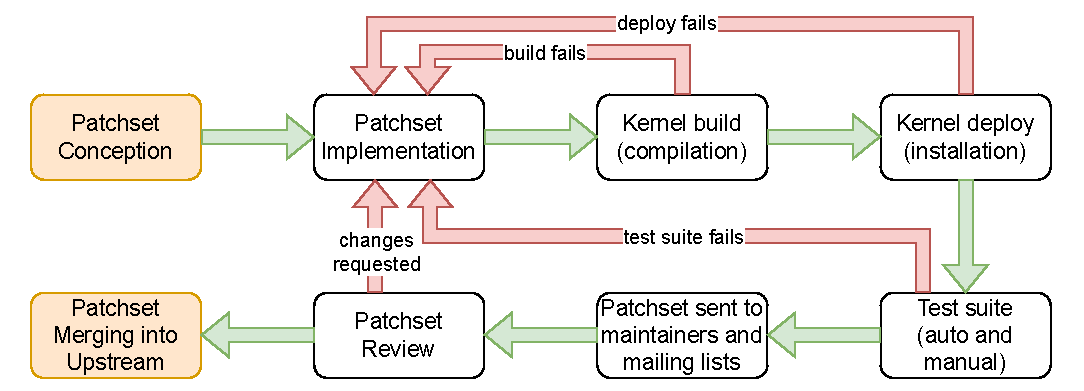
\includegraphics[width=1\linewidth, 
    clip=true, trim= 0px 0px 0px 0px]
    {figs/patchset-development-workflow.pdf}}
    \caption{Concept map of the patchset development workflow.}
    \label{fig:patchset-dev-workflow}
\end{figure}

\begin{figure}[ht]
    \centering
    \fbox{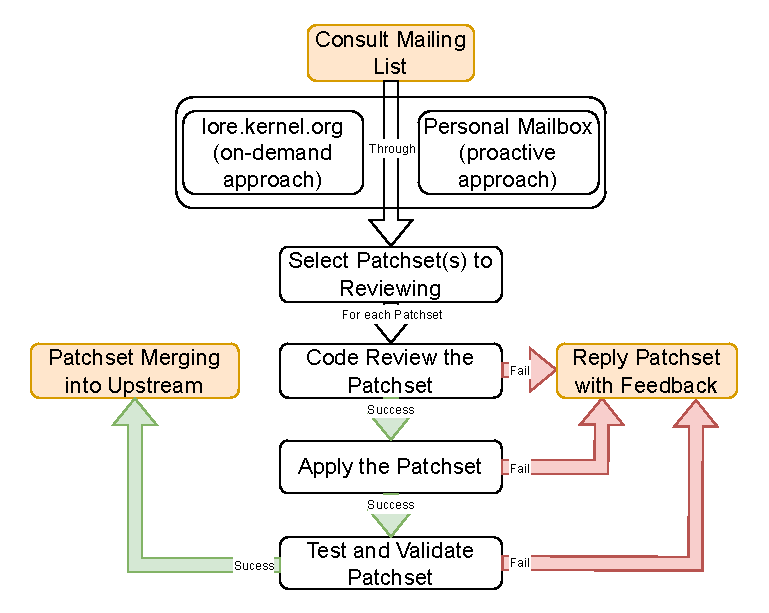
\includegraphics[width=1\linewidth, 
    clip=true, trim= 0px 0px 0px 0px]
    {figs/patchset-reviewing-workflow.pdf}}
    \caption{Concept map of the patchset reviewing workflow.}
    \label{fig:patchset-dev-workflow}
\end{figure}

\section{Kworkflow}

\texttt{Kworkflow}~\cite{kworkflow} (kw) is a \textit{Developer Automation
Workflow System} (DAWS) that targets Linux kernel developers. kw is a FLOSS
project licensed under the \textit{GNU General Public License version 2}
(GPLv2).

Generally, any developer who needs to work with the Linux source code can
benefit from using kw. For instance, in the GNU/Linux distribution (also called
\textit{distro}) layer, distro developers feed off the official releases (the
\textit{upstream} git repository) and maintain their own kernel tree (a
\textit{downstream} git repository) where they add their specific modifications
to the source code, occasionally returning contributions to the upstream. No
matter if they engage or not in the Linux project development, these developers
must also configure, build, deploy, and the like, making kw an interesting
choice.

kw aims to streamline and automate kernel workflows by offering a diverse set of
commands in a unified CLI that helps users to manage \texttt{.config} files,
build and deploy kernels, manage virtual and network-accessible machines,
seamlessly send patches in compliance with Linux guidelines, and more. Through
Bash script, kw leverages the \textit{GNU coreutils} and other CLI tools to
create solutions with sane basic configurations that offer a
\textit{plug-n-play} experience without limiting customization.

\subsection{Installation}

Currently, the best way to install kw is by cloning the project locally with
\texttt{git} and running the \texttt{setup.sh} script~\cite{kworkflow-setup}
with the \texttt{--install} option. After running the script, the user will be
prompted for superuser credentials to install the necessary dependencies using
the appropriate package manager (\texttt{apt}, \texttt{pacman}, \texttt{dnf},
etc.), then the script installs kw files in the user's system. \textbf{Listing
\ref{lst:kw-setup}} illustrates the mentioned steps.

\begin{lstlisting}[caption={Installing kw via the \texttt{setup.sh} script.}, label={lst:kw-setup}]
$ git clone https://github.com/kworkflow/kworkflow
$ cd kworkflow
$ ./setup.sh --install
\end{lstlisting}

\subsection{Features}

Once installed, kw offers a significant number of commands (features) that can
be invoked as described in \textbf{Listing \ref{lst:kw-commands}}. Features of
kw can be categorized depending on their purpose, and \textbf{Table
\ref{tab:kw-commands}} lists all features with their categories and
descriptions.

\begin{lstlisting}[caption={kw commands invocation.}, label={lst:kw-commands}]
$ kw <command> <options/arguments>
\end{lstlisting}

\begin{table}[ht]
    \caption{kw commands}
    \label{tab:kw-commands}
    \begin{center}
    \begin{tabular}{|p{0.2\columnwidth}|p{0.30\columnwidth}|p{0.40\columnwidth}|}
        \hline
        \rowcolor{gray!20}
        \textbf{Command} & \textbf{Category} & \textbf{Description} \\\hline
        \texttt{build}    & kernel build/deploy    & Build kernel and modules \\\hline
        \texttt{deploy}    & kernel build/deploy    & Deploy kernel and modules \\\hline
        \texttt{kernel\-config\-manager}    & kernel build/deploy    & Manage \texttt{.config} files \\\hline
        \texttt{env}    & kernel build/deploy    & Manage different environments for same kernel tree \\\hline
        \texttt{bd}    & kernel build/deploy    & Build and Deploy kernel and modules \\\hline
        \texttt{send-patch}    & patch submission    & Send patches via email \\\hline
        \texttt{maintainers}    & patch submission    & \texttt{get\_maintai\-ners.pl} wrapper \\\hline
        \texttt{codestyle}    & patch submission    & \texttt{checkpatch.pl} wrapper \\\hline
        \texttt{remote}    & target machine    & Manage machines in the network \\\hline
        \texttt{vm}    & target machine    & QEMU wrapper \\\hline
        \texttt{ssh}    & target machine    & \texttt{ssh} wrapper \\\hline
        \texttt{device}    & target machine    & Show hardware information \\\hline
        \texttt{debug}    & code inspection    & Linux debug utilities \\\hline
        \texttt{explore}    & code inspection    & Explore string patterns \\\hline
        \texttt{diff}    & code inspection    & Diff files \\\hline
        \texttt{init}    & kw management    & Initialize kw kernel tree \\\hline
        \texttt{config}    & kw management    & Set kw configs \\\hline
        \texttt{self-update}    & kw management    & Self-update mechanism \\\hline
        \texttt{backup}    & kw management    & Save and restore kw data \\\hline
        \texttt{clear-cache}    & kw management    & Clear kw cache \\\hline
        \texttt{patch-hub}    & misc    & TUI for patches from lore.kernel.org \\\hline
        \texttt{drm}    & misc    & DRM specific utilities \\\hline
        \texttt{pomodoro}    & misc    & Pomodoro technique \\\hline
        \texttt{report}    & misc    & Show usage statistics \\\hline
    \end{tabular}
    \end{center}
\end{table}

In the remainder of this section, we will deep dive into some of the kw
features, their use cases and highlight interesting aspects of each.
Nevertheless, \textbf{keep in mind} that kw does a lot more than what is
showcased next.

\subsubsection{kw build}

The \texttt{build} command, along with \texttt{deploy}, are the flagship
features of kw and probably the most elaborate ones. As mentioned in
\textbf{Section~\ref{sec:background:linux-tasks}}, building a kernel is not an
easy task, even when you have a \texttt{.config} ready. \textit{GNU make} (the
\texttt{make} utility) immensely helps in this task; nevertheless, one would
still have to keep in mind the target architecture, cross-compilation (if
needed), the number of CPU cores allocated, which \texttt{KCFLAGS} (short for
\textit{kernel compiler flags}) to use, and so on.

\begin{lstlisting}[caption={Example of kernel build \texttt{make} command.}, label={lst:classic-build-example}]
$ make ARCH=arm64 CROSS_COMPILE=aarch64-linux-gnu- -j8 'KCFLAGS=-DNICE_MACRO'
\end{lstlisting}

For instance, say the user wishes to build a kernel from an x86\_64 host to an
ARM64 target machine using all his CPU cores (eight cores available) while
defining a macro called \texttt{NICE\_MACRO}. Assuming that the necessary
\texttt{.config} is in place, \textbf{Listing~\ref{lst:classic-build-example}}
shows a \texttt{make} command for this scenario. 


In comparison, after a one-time simple setting of the aforementioned information
using the kw command \texttt{config} (as it will be described), the user only
needs to issue the command in \textbf{Listing~\ref{lst:kw-build-example}}.

\begin{lstlisting}[caption={\texttt{kw build} use case.}, label={lst:kw-build-example}]
$ kw build
\end{lstlisting}

The \texttt{build} command offers many options that go beyond simply automating
the equivalent \texttt{make} commands, namely: \texttt{--info} that displays
information about the current compilation with kernel name and number of modules
to be compiled; \texttt{--llvm} that enables use of the LLVM toolchain; and
\texttt{--from-sha} that builds every commit version of the kernel from a
\texttt{git} reference passed as an argument.

\subsubsection{kw deploy}

Although much less demanding regarding resources than building, deploying a
kernel can be more complicated and detail-filled than compiling. Simply put, the
task involves copying the necessary compiled artifacts to the correct place with
the correct name in the target machine's filesystem, defining a temporary
filesystem needed for the kernel to boot the system, and updating the
bootloader. Apart from these being non-trivial steps, these steps can also
mutate quite a lot depending on the target machine CPU architecture, Linux
distro, and many other factors.

The \texttt{deploy} command absorbs most of these complexities in its code, so
users do not need to configure most of the steps, with the feature detecting
information about the target machine and resolving the details. Unlike the pair
of \textbf{Listing~\ref{lst:classic-build-example}} and
\textbf{Listing~\ref{lst:kw-build-example}}, an equivalent series of commands
that would represent a single \texttt{kw deploy} call would involve many
commands (in the range of dozens) that are extensive, so presenting a comparison
here would only produce visual pollution. This speaks in favor of how well
\texttt{deploy} not only automates but streamlines the task of installing
kernels.\looseness=-1

Like with \texttt{build}, \texttt{deploy} has options that offer other
enhancements, like: \texttt{--list} to list installed kernels in a target
machine; \texttt{--uninstall} to uninstall kernels and related artifacts; and
\texttt{--create\-package} and \texttt{--from-package} to generate a compressed
file that can be transported offline (in a USB device, for instance) and be used
to deploy the kernel on another machine, which only has to have kw installed.\looseness=-1

\subsubsection{bd}

Because deploying a kernel often comes right after building it, kw offers the
\texttt{bd} command (from \textit{build and deploy}) to chain the two previously
mentioned features, optimizing even more the task of booting a kernel built from
the source code.

\subsubsection{kernel-config-manager}

Automating and streamlining the automation of a \texttt{.config} file that is
the perfect fit for a developer use case is an open problem, with some attempts
to solve this in the context of Linux CI~\cite{yildiran2024maximizing}. As such,
kw still does not cover the generation part, but offers a very comprehensive
feature, \texttt{kernel\-config-manager}, for users to easily keep records of a
great variety of \texttt{.config} files. The feature works differently depending
on the subcommand used: \texttt{--save} saves the current \texttt{.config} with
a name and an optional description; \texttt{--get} restores a saved
\texttt{.config} of the name passed as argument; and \texttt{--remove} removes
the entry related to the name passed as argument.

\begin{lstlisting}[caption={\texttt{kw kernel-config-manager} use case.}, label={lst:kw-k-example}]
$ kw k --save foo --description 'bar'
$ kw k --get foo
$ kw k --remove foo
\end{lstlisting}

\textbf{Listing~\ref{lst:kw-k-example}} exemplifies these three subcommands
usage (note that we use the short name \texttt{k} of the feature for
readability). \textbf{Figure 5} is a screen capture that showcases another
subcommand, \texttt{--list}, that lists all \texttt{.config} files managed by
the feature.

\begin{figure}[htbp]
    \centering
    \fbox{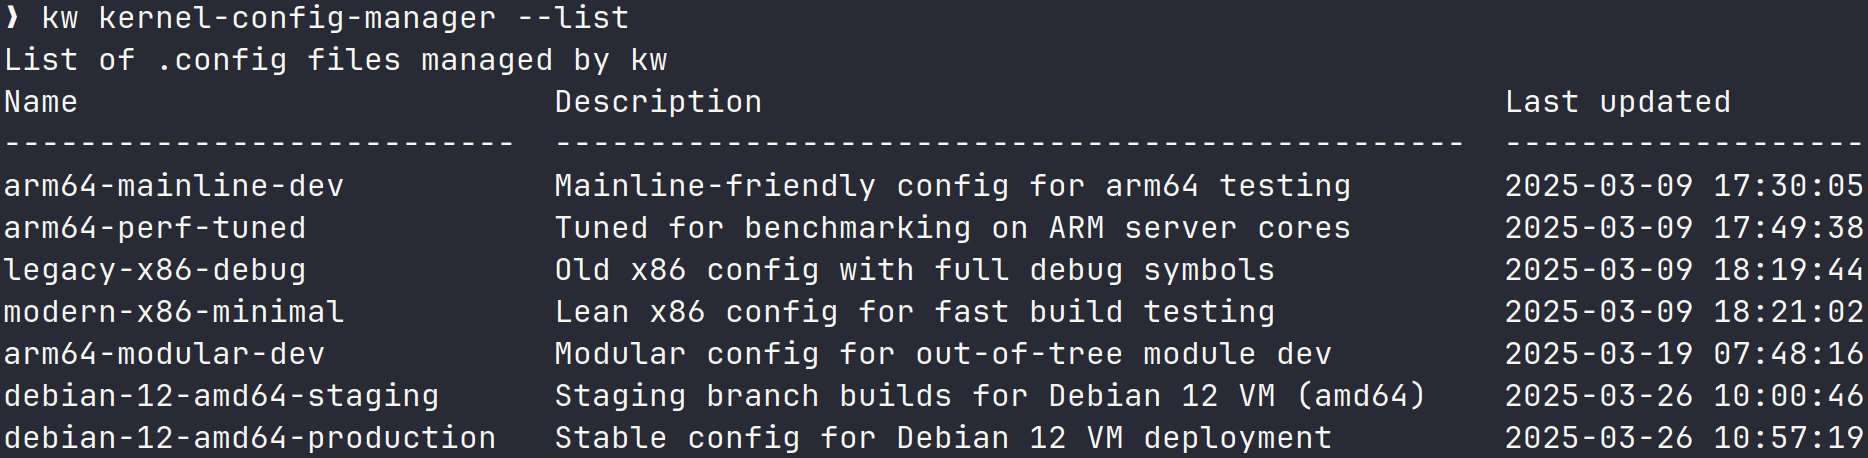
\includegraphics[width=1\linewidth, 
    clip=true, trim= 0px 0px 0px 0px]
    {figs/kw_k_list_example}}
    \caption{\texttt{kw kernel-config-manager --list} example.}
    \label{fig:patchset-dev-workflow}
\end{figure}

\subsubsection{env}

The result of building the kernel, i.e., the object files and related artifacts,
by default, resides in the same kernel tree used for the source code of the
compilation. However, some developers need to build kernels for different
targets from the same kernel tree, which becomes unmanageable as the number of
targets rises, due to the need for multiple \texttt{.config} files, build
configurations, and more.\looseness=-1

\begin{lstlisting}[caption={\texttt{kw env} use case.}, label={lst:kw-env-example}]
$ kw env --create FOO
$ kw env --use FOO
$ kw env --destroy FOO
\end{lstlisting}

To solve this problem, the \texttt{env} command allows users to create different
environments that isolate development contexts using a single kernel tree. The
corresponding files are stored inside a cache directory that is managed by kw.
With the use of the subcommands \texttt{--create}, \texttt{--use}, and
\texttt{--destroy}, users can manage their environments
(\textbf{Listing~\ref{lst:kw-env-example}}), and with \texttt{--list} consult
their environments (\textbf{Figure 6}).

\begin{figure}[htbp]
    \centering
    \fbox{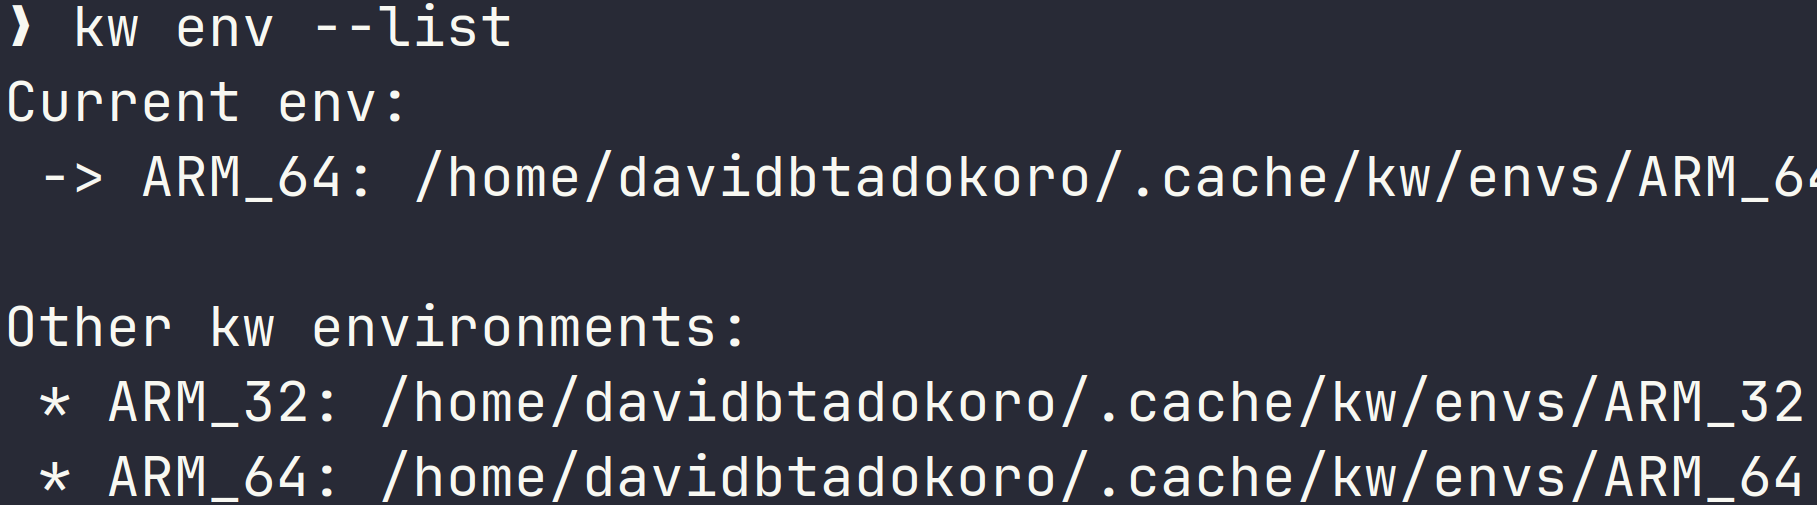
\includegraphics[width=0.8\linewidth, 
    clip=true, trim= 0px 0px 0px 0px]
    {figs/kw_env_list_example}}
    \caption{\texttt{kw env --list} example.}
    \label{fig:patchset-dev-workflow}
\end{figure}

\subsubsection{send-patch}

The act of converting a commit or set of commits into patches and sending them
through email is vastly covered by the \texttt{git-send-email} tool. However, it
can be considered raw from the point of needing a lot of configuration, verbose
commands, and, mainly, a lack of integration with the
\texttt{get\_maintainers.pl} tool. This last problem forces users to manually
resolve and add the correct recipients. The \texttt{send-patch} command solves
all three by providing default base configurations, shorter commands, and
automatically resolving recipients.
\textbf{Listings~\ref{lst:git-send-email-example}} and
\textbf{\ref{lst:kw-send-patch-example}} show, respectively, a
\texttt{git-send-email} command to send the current commit explicitly stating
the recipients with additional options and the respective \texttt{send-patch}
command.

\begin{lstlisting}[caption={Example of \texttt{git-send-email} command.}, label={lst:git-send-email-example}]
$ git send-email -1 --annotate --to=foo@bar.com --cc=bar@foo.com
\end{lstlisting}

\begin{lstlisting}[caption={\texttt{kw send-patch} use case.}, label={lst:kw-send-patch-example}]
$ kw send-patch --send
\end{lstlisting} 

\subsubsection{config}

Having a plethora of features, kw has its own system to manage the
configurations of each and a dedicated feature for users to interface with. The
syntax of the \texttt{config} feature is composed of the pair
\texttt{feature.configuration} followed by the value wished to be bound to the
configuration. For example, \textbf{Listing~\ref{lst:kw-config-example}}
illustrates a case of configuring the target architecture of the \texttt{build}
command to be x86\_64.

\begin{lstlisting}[caption={\texttt{kw config} use case.}, label={lst:kw-config-example}]
$ kw config build.arch 'x86_64'
\end{lstlisting}

\subsubsection{patch-hub}

A singular feature of kw is \texttt{patch-hub} as it is a sub-project with a
dedicated git repository, is written in Rust, and is a \textit{Terminal User
Interface} (TUI), a text-based equivalent of a \textit{Graphical User Interface}
(GUI) which significantly diverges from the fully CLI approach of the rest of
kw. Nonetheless, it still provides interesting services to kernel developers,
specifically the maintainers, as the feature is a TUI that allows users to
consult the flow of patches in lore.kernel.org, apply actions on them using
other kw features, and more. The feature aims to cover the patchset reviewing
workflow described in \textbf{Figure 2}. \texttt{patch-hub} has a lot more
capabilities and is a work-in-progress, but \textbf{Figure 5} gives an overview
of the potential of the feature.

\begin{figure}[htbp]
    \centering
    \fbox{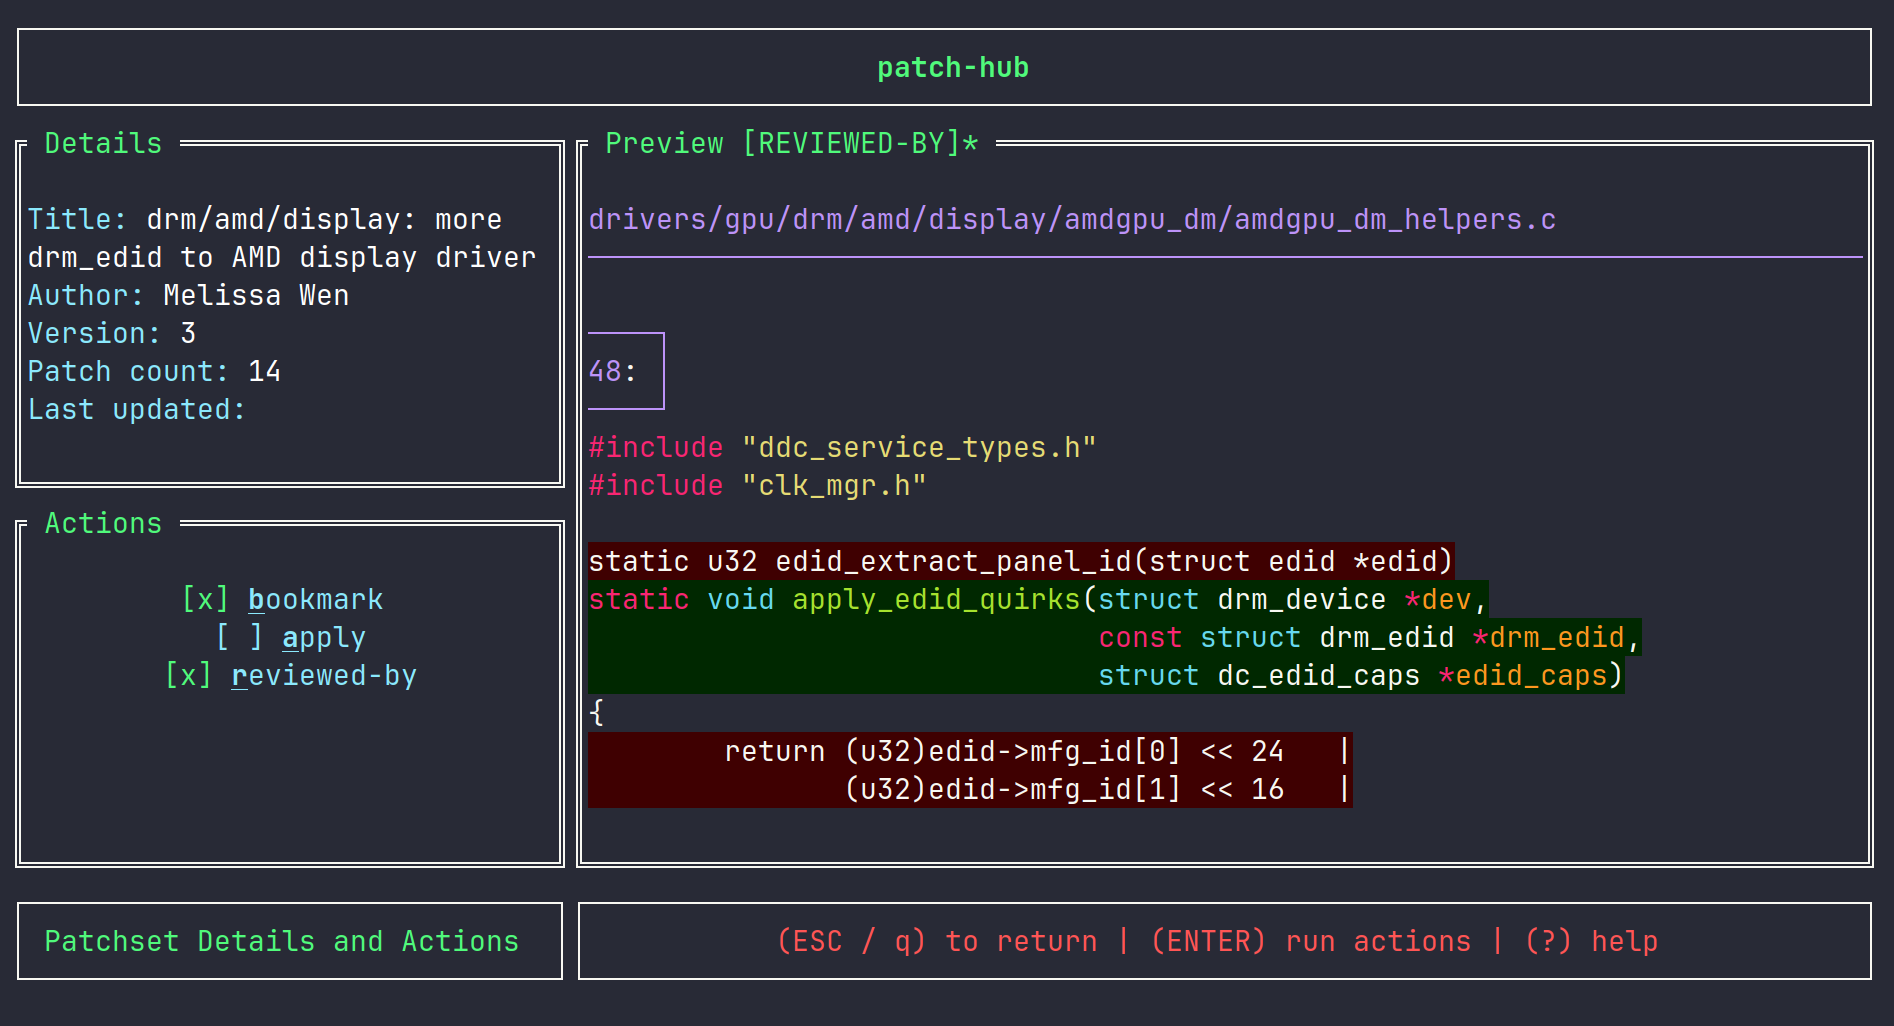
\includegraphics[width=1\linewidth, 
    clip=true, trim= 0px 0px 0px 0px]
    {figs/kw_patch_hub_example}}
    \caption{\texttt{kw patch-hub} use case.}
    \label{fig:patchset-dev-workflow}
\end{figure}

\subsection{Project architecture}

Describing kw as hub-like fits not only from the user's perspective, as it is a
collection of diverse features in a unified interface, but also from the project
developer's perspective. The project code base is structured as follows:

\begin{enumerate}
	\item Entry point file named \texttt{kw} located at the root of the
	repository~\cite{kworkflow-entrypoint}, that is our \textit{hub} component;
	\item Feature-specific files named after their respective feature (e.g., the
	\texttt{build} feature has the \texttt{build.sh} file) located at the
	\texttt{src/} directory~\cite{kworkflow-features}. These are our
	\textit{features} components;
	\item Library files named after their scope (e.g., \texttt{kw\_string.sh}
	deals with string manipulations) located at the \texttt{src/lib/}
	directory~\cite{kworkflow-libraries}, that are shared across
	feature-specific files. These are our \textit{libraries} components;
	\item Plugin files with code heavily coupled with specific distros, CPU
	architectures, subsystems, and the like, that can change externally and are
	very mutable, located at the \texttt{src/plugins/}
	directory~\cite{kworkflow-plugins}.  These are our \textit{plugins}
	components
\end{enumerate}


As an illustration of kw's inner workings, let us simulate an execution of a
\texttt{kw deploy} call. First, the entry point \texttt{kw} file is loaded and
executed. At the beginning, global variables are dynamically defined, then using
a switch-case, we resolve the feature as \texttt{deploy}, load the
\texttt{deploy.sh} file, and call the standard main function of feature-specific
files (in this case, \texttt{deploy\_main()}). This function handles the rest of
the \texttt{deploy} execution, using other functions defined inside
\texttt{deploy.sh} and leveraging functions from the libraries and plugins
components.

\begin{figure}[htbp]
    \centering
    \fbox{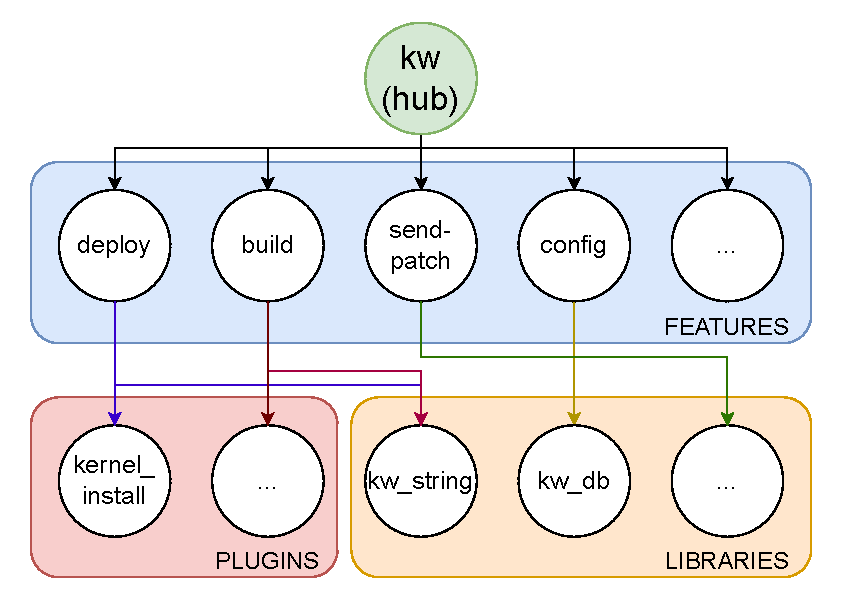
\includegraphics[width=0.8\linewidth, clip=true, trim= 0px 5px 0px 5px]
    {figs/kw-architecture.pdf}}
    \caption{kw conceptual architecture.}
    \label{fig:kw-arch}
\end{figure}

The diagram in \textbf{Figure~\ref{fig:kw-arch}} models kw's architecture
showing how extensible and modularized the project is. Note that this diagram is
for illustration purposes and does not reflect the precise load and execution
relation of features and libraries/plugins.

\subsection{Data collection for scientific research}

Inside the kw project, we have implemented an infrastructure to collect
statistics and other data, along with a lightweight and single-file database
using \textit{SQLite3}~\cite{sqlite}. For instance, every time a developer builds
a kernel, the time it took for the compilation is captured (using the
\texttt{statistics} library) and registered in kw's database (using the
\texttt{kw\_db} library). This type of data collection happens in other places
across kw, but many other data points opportunities can be used to conduct
further scientific research on kernel workflows.

To name a few, kw captures: build and deploy times, logging if they were
successful; target machine kernel list and uninstall events. We can also list
some data points of interest in terms of research on the kernel workflows:
during build, capture hardware specifications and cross-compilation strategies,
enabling analysis of efficient hardware setups and common compiler use; during
deployment, record target distro, bootloader, and deployment method, which can
uncover the landscape in terms of testing environments used; during patch
submission log maintainer/mailing list targeting, providing insights about
overloaded personell/subsystems in the Linux project hierarchy.

All data is stored locally in a single file within the user's file system, never
exfiltrated, and users can easily opt out by disabling data collection. We also
plan to implement a telemetry system for users to voluntarily submit data for
research, inspired by the \textit{Debian Popularity
Contest}~\cite{debian-popcon}, a standard in telemetry and anonymization.

\subsection{Comparison with other tools}

kw works as a hub-like tool that continuously incorporates existing robust tools
to avoid duplication, while also implementing features from scratch when no
existing tools (satisfiably) solve a given pain point. Incorporating other tools
involves adding our biases, which we believe are closely tied to the Linux
kernel development model rules and workflows. In this respect, no other tool
exists that proposes a similar all-in-one approach to mitigate bottlenecks in
kernel workflows, making kw a novel solution.


\section{Conclusion}

Kworkflow (kw) automates and streamlines kernel workflows by leveraging existing
solutions fragmented across the Linux ecosystem and presenting a cohesive and
unified CLI to users. The tool abstracts complexity in tasks such as build,
deploy, and patch submission, mitigating bottlenecks in development, and
supporting the long-term sustainability of Linux, while reducing duplication of
efforts and wasted resources by the community. As a hub-like solution, kw is
built to be extensible and modularized, allowing continuous incorporation of
other tools to cover more kernel developers' pain points. Beyond its immediate
utility, kw presents an incredible and robust opportunity for data collection
that can further scientific research in the Linux kernel development model.


\section*{Artifacts Availability}

\begin{itemize}
  \item kw official repository: \url{https://github.com/kworkflow/kworkflow}
  \item kw Software Heritage archive: \url{https://archive.softwareheritage.org/browse/origin/directory/?origin_url=https://github.com/kworkflow/kworkflow}
  \item kw website: \url{https://kworkflow.org}

\end{itemize}

\begin{acks}
  This study was financed, in part, by CAPES (Finance Code 001), the University of São Paulo – USP (Proc. 22.1.9345.1.2), the São Paulo Research Foundation – FAPESP (Proc. 19/26702-8) and the São Paulo State Data Analysis System Foundation – SEADE (Proc. 2023/18026-8), Brazil. We also thank the community for collaboratively building and maintaining kw, members of the Linux ecosystem for the feedback provided, and the students from IME-USP who have voluntarily fostered the project throughout the years.
\end{acks}

%%
%% The next two lines define the bibliography style to be used, and
%% the bibliography file.
\bibliographystyle{ACM-Reference-Format}
\bibliography{references}

\end{document}
\endinput
